\subsection*{Question 3.3}
In this question we are using these 2 equations:

\begin{equation}
	u = \frac{1}{\sqrt{\lambda_1}}k^T_1(s-\mu)
\end{equation}

\begin{equation}
	v = \frac{1}{\sqrt{\lambda_1}}k^T_1(s-\mu)
\end{equation}

$k_1$ and $k_2$ are the eigenvectors for the two best eigenvalues. We make a scatter plot over the differences as indicated by the two eigenvectors (see figure \ref{fig:q33scatter}), where values of 0 in the x and y axes is the solution closest to the mean hand. It can also be seen that most of the hands lay pretty close to the x axis.

\begin{figure}[!htbp]
  \centering
  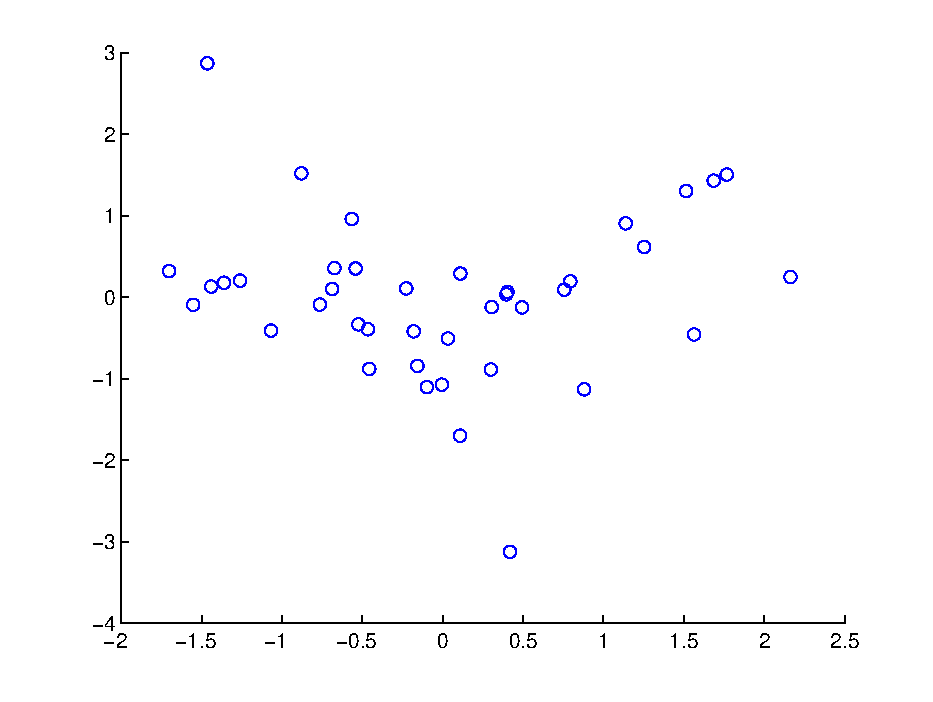
\includegraphics[width=0.85\textwidth]{./images/q33_scatter}
  \caption{A scatter plot of the hands variation as indicated by the eigenvectors of the two largest eigenvalues.}
  \label{fig:q33scatter}
\end{figure}

Measuring the distance from the center, we see that the 5 largest distances are\\$d = [3.2194, 3.1527, 2.3197, 2.2101, 2.1770]$.
Notice that two of these have significantly larger values than the following.
Looking at the plot, we also notice that two points are significantly futher from the others.
The hands corresponding to these points are seen in figure \ref{fig:q33}, where we can see that they are, indeed, differing from the mean hand.

\begin{figure}[!htbp]
  \centering
  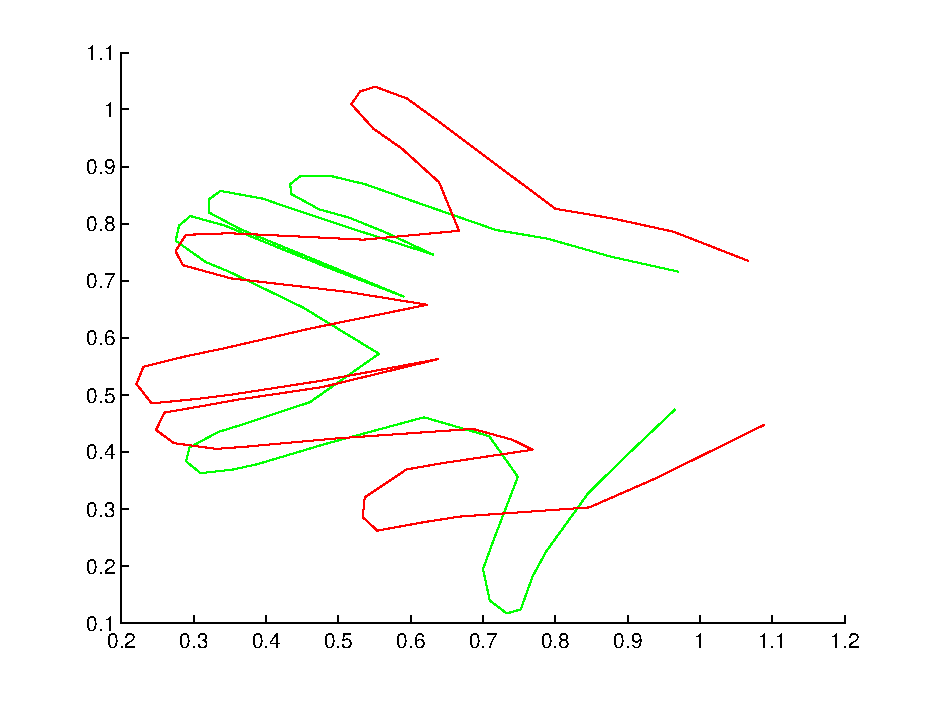
\includegraphics[width=0.85\textwidth]{./images/q33}
  \caption{The two hands that are the worst fits to the mean hand. Distance-wise, the the green hand is the worst, and the red is the second worst.}
  \label{fig:q33}
\end{figure}
